\chapter{Geoid prediction}\label{chap:content}

To explore the the potential use of neural networks in forward modelling a geoid surface, we use a 1D spherically symmetric viscosity model to compute a geoid surface in terms of some spherical harmonics coefficients that can be used to construct the Geoid surface. To further simplify this problem, the data set used for this research uses a reduced
prior such that the perturbations to the output are smaller.


\section{Dataset of Geoid prediction}

The reduced data set consists of 1000 pairs of input and output. In the data set, input is a vector with 257 values indicating a 1D spherically symmetric viscosity model and output is a vector with 60 values representing a set of spherical harmonic coefficients describing the geoid height on the surface of the Earth. The following figure is a sample visualization of a random set of 60 geoid coefficients from the output data as a 2D image, where this set of coefficients basically map to an image wrapped on the surface of a sphere.

\begin{figure}[H]
    \caption{Sample Geoid Coefficients Visualization,  where the units of the geoid are in metres and 
     represent values greater or less than some reference value.}
    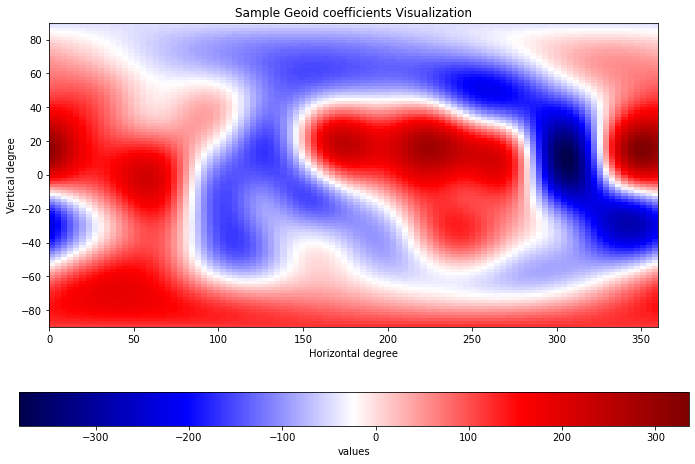
\includegraphics[scale=0.6]{figures/geoid_images/Geoid_Sample_visualization.png}
\end{figure}

To further observe the patterns in the input and the output, 10 pairs of model input and output are plotted in the following figures.

\begin{figure}[H]
    \caption{Every 100th input in the data set.}
    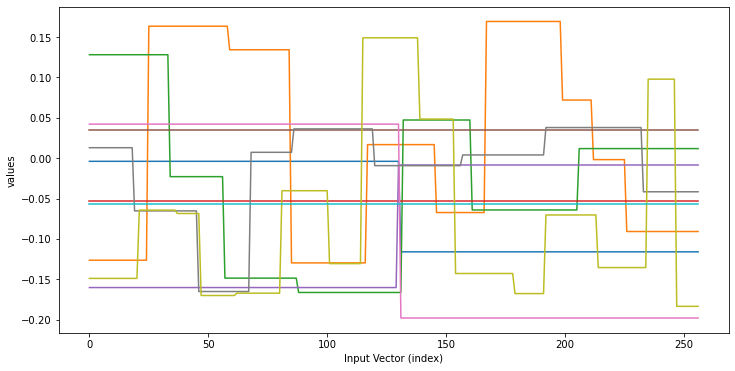
\includegraphics[scale=0.6]{figures/geoid_images/Geoid_sample_input.png}
\end{figure}

\begin{figure}[H]
    \caption{Every 100th output in the data set.}
    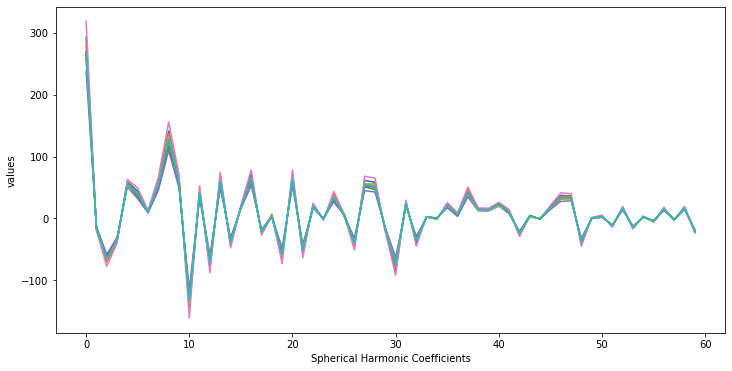
\includegraphics[scale=0.6]{figures/geoid_images/Geoid_sample_output.png}
\end{figure}

From the second plot we can observe that the outputs in the data set can be seen as some "curves" with the same patterns but different altitude. In this case, each of the 60 coefficients in the output data are normalised to be between 0 and 1 using their maximum and minimum values separately before feeding into the neural network. This is because each of the parameters in an output vector can be seen as equal and we want to prevent the neural network from spending most of its effort learning the parameter with a higher range. Hence, one can expect a higher accuracy when the parameters in the output data are standardized to a same range.

After the output data is normalised using a scaler, the entire data set is randomly divided in a ratio of 8:1:1: 80 per cent of the data set is used for training, 10 per cent of the data for testing accuracy and the remaining 10 per cent to perform validation during training and prevent overfitting. For a data set with 1000 samples, this result in a train-test-valiadation split of 800-100-100.


\section{Fully connected Neural Network (FNN) for Prediction}

To test FNNs with different architectures (e.g. different number of hidden layers and neurons per hidden layer) or other hyperparameters (e.g. optimizer), a systematic testing method is applied. This method mainly consists of three files: one file to store all the different set of FNN architectures and hyperparameters in a text format, another file to fetch all these combinations of architectures and hyperparameters line by line, build them as FNN models and train these models, and the last file for testing and visualisation of the trained models by specifying the path of the trained model. The training file and the testing file are both in the format of a Jupyter Notebook.

The trained FNN architecture (in the format of a light-weight file) along with another text file contains the training loss and validation loss during training will be stored in a specified path for further testing and visualisation. The name of these two files uniquely defines each experiment by including the values of hyperparameters to generate the model in the file names. These files are also put in separate folders with the folder name associated with commit IDs to handle tracking of the process during the research in an educated or extensible way.

In this way, one can open the same testing Jupyter Notebook in different browser tabs, and then visualize simultaneously different models in different tabs using a cell in which the paths to the FNN file and its training data are specified. 

The systematic testing capability is implemented here to ensure traceability. In other words, as different values of the hyperparameters are tested, We would like to be able to record the results (e.g., the trained network and the training data) so that we don't have to repeat them again or rely on our memory to compare the the performance of different structures.

Also, to prevent overfitting, a variation of the early-stopping method is used during training. The normal early-stopping method let the network train until the error function evaluated on the validation set starts to increase beyond a certain threshold\citep{10.1007_978-3-642-35289-8_5}, while my implementation only stores the best model during training (the one with the lowest validation loss) in a specified path and allows the network to keep training as normal. In this case, the output model is the best model instead of the last trained model. This method is also used in the following chapter when implementing the ConvAE, FNN and LSTM to solve the mantle convection problem.

After testing with NNs with architectures of different number of hidden layers and neurons per hidden layer, we found that architectures with a total number 3–4 hidden layers seemed to perform the best.

In the following figures, we present results from a FNN with 4 hidden layers with 200, 160, 120 and 80 neurons, ReLU as activation function, MSELoss as loss function, and trained for 200 epochs using Mini-Batch Gradient Descent (with a batch size of 16).

One thing to notice is that the loss value that is back-propagated during the training process is calculated using the prediction and the normalised output. In this case, the best case and the worst case shown as below are also defined upon the value of this normalised error in order to be consistent.

\begin{figure}[H]
    \caption{Training loss and Validation loss.}
    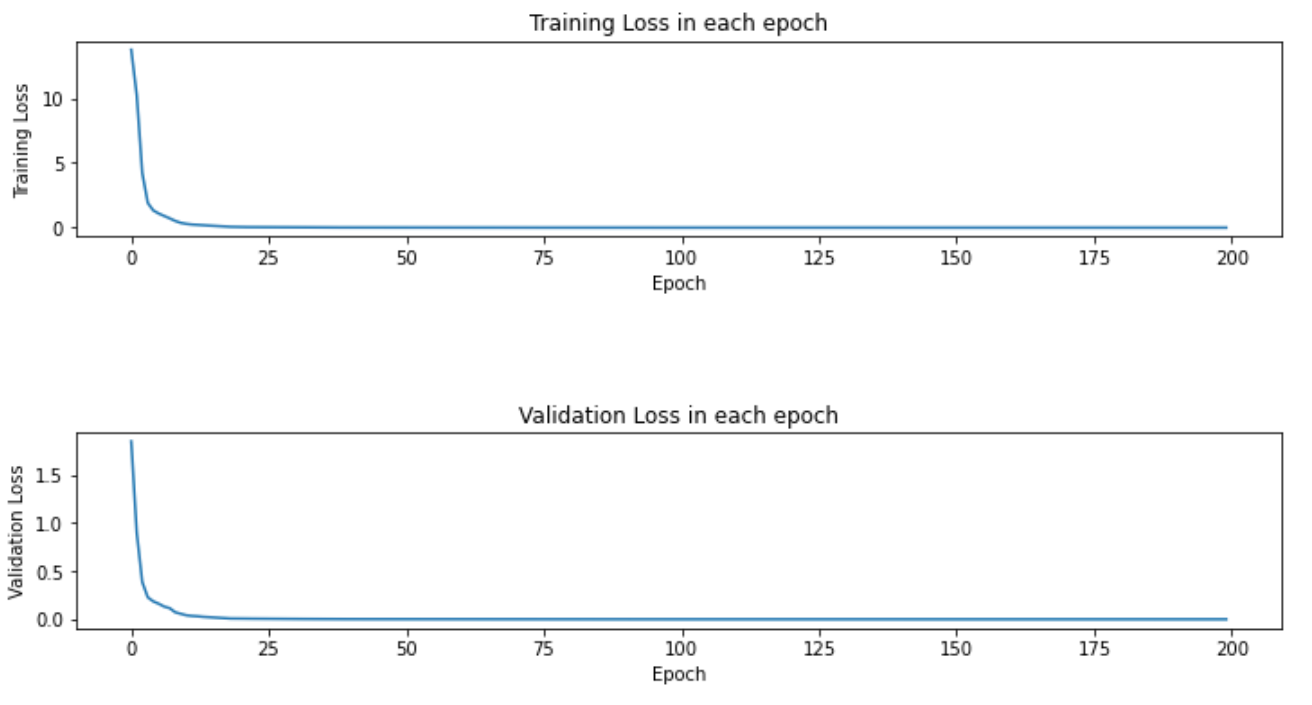
\includegraphics[scale=0.6]{figures/geoid_images/Geoid_trainingData.png}
\end{figure}

\begin{figure}[H]
    \caption{Overall testing result.}
    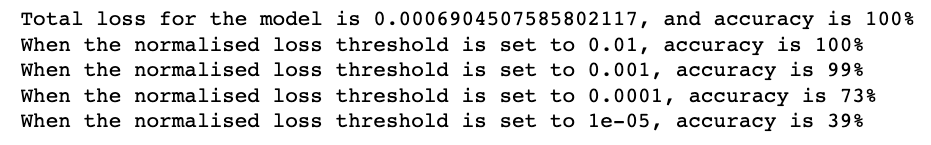
\includegraphics[scale=0.8]{figures/geoid_images/Geoid_OverallTesting.png}
\end{figure}

\begin{figure}[H]
    \caption{Most accurate Geoid prediction.}
    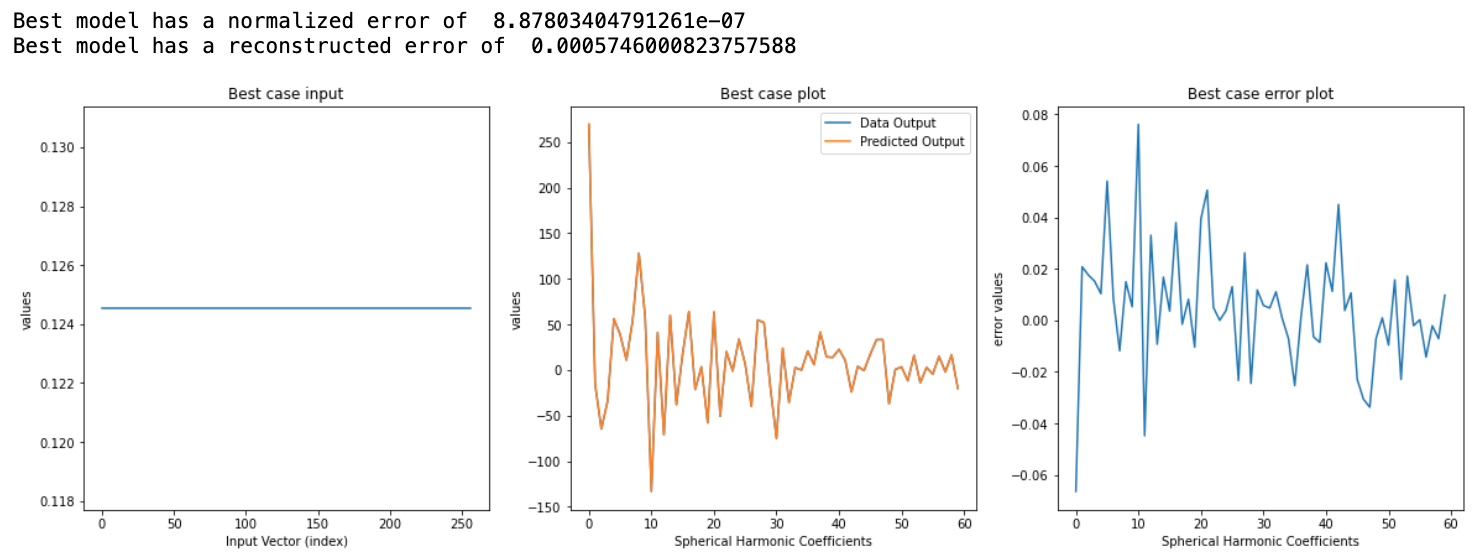
\includegraphics[scale=0.6]{figures/geoid_images/Geoid_Best.png}
\end{figure}

\begin{figure}[H]
    \caption{Least accurate Geoid prediction.}
    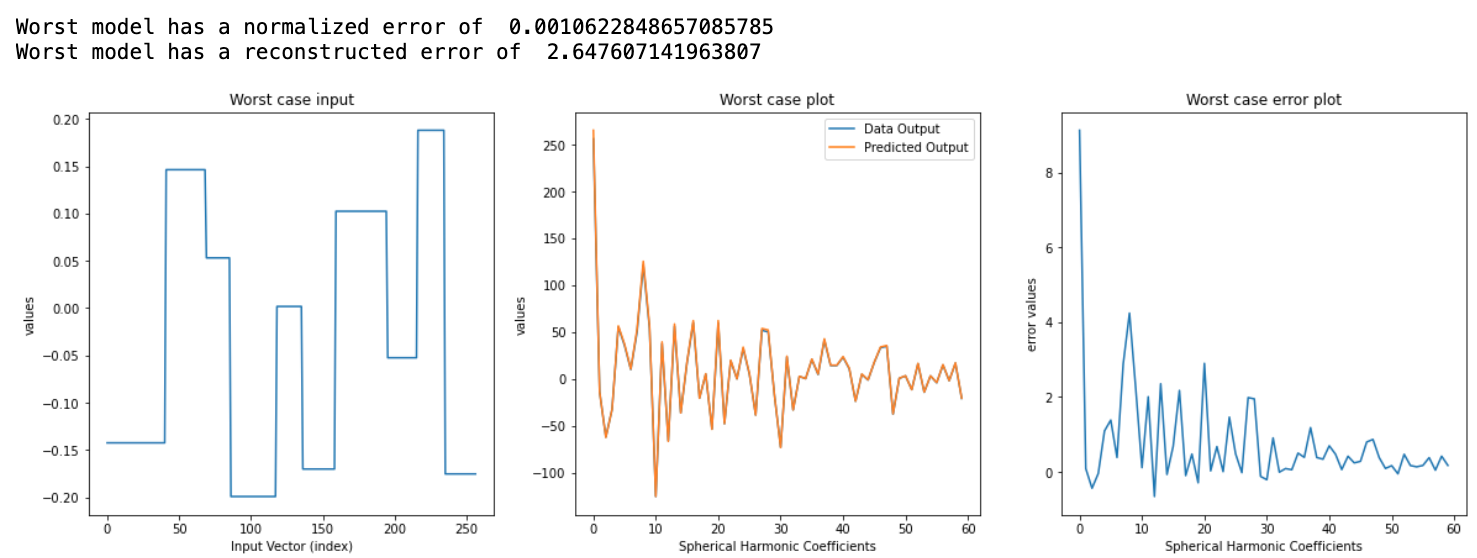
\includegraphics[scale=0.6]{figures/geoid_images/Geoid_Worst.png}
\end{figure}

On average, both the normalised loss and the reconstructed loss are low and no overfitting occurs. The accuracy of the prediction is nearly 100\% when the threshold is set to be 10 times lower than the worst loss value. 

For further testing, the set of 60 coefficients produced by the FNN in both the best case and the worst case are visualized on globe geoid maps that are flattened as a 2D images, along with the map of the actual output data and an error map representing the difference between the prediction and the ground truth.

\begin{figure}[H]
    \caption{Visualization of the most accurate Geoid prediction.}
    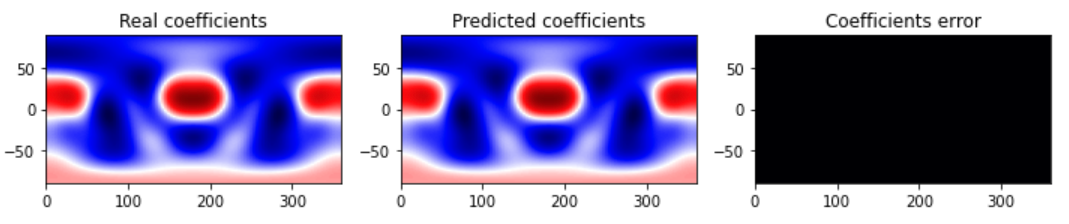
\includegraphics[scale=0.4]{figures/geoid_images/Geoid_Best_visualization.png}
\end{figure}

\begin{figure}[H]
    \caption{Visualization of the least accurate Geoid prediction.}
    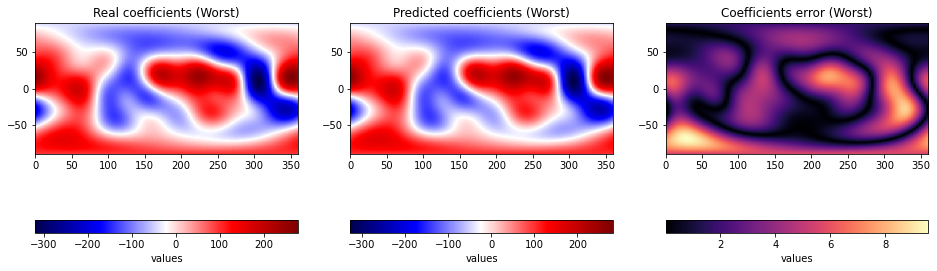
\includegraphics[scale=0.4]{figures/geoid_images/Geoid_Worst_visualization.png}
\end{figure}

We can observe that the result produced by the FNN is in high quality even in the worst case.

Overall, FNN is able to accurately solve the Geoid problem without numerous amount of data.


